Auf folgenden Seiten sind ausgewählte, vorher dargestellte UML Diagramm vergrößert abgebildet.

\begin{figure}[h!]
	\centering
	\includegraphics[height=\textwidth, width=\textheight, keepaspectratio=true, angle=90]{dia/TwitterGUI_Erweiterung}
	\caption{Größeres Klassendiagramm der GUI}
	\label{fig:gui_big}
\end{figure}
\begin{figure}[h!]
	\centering
	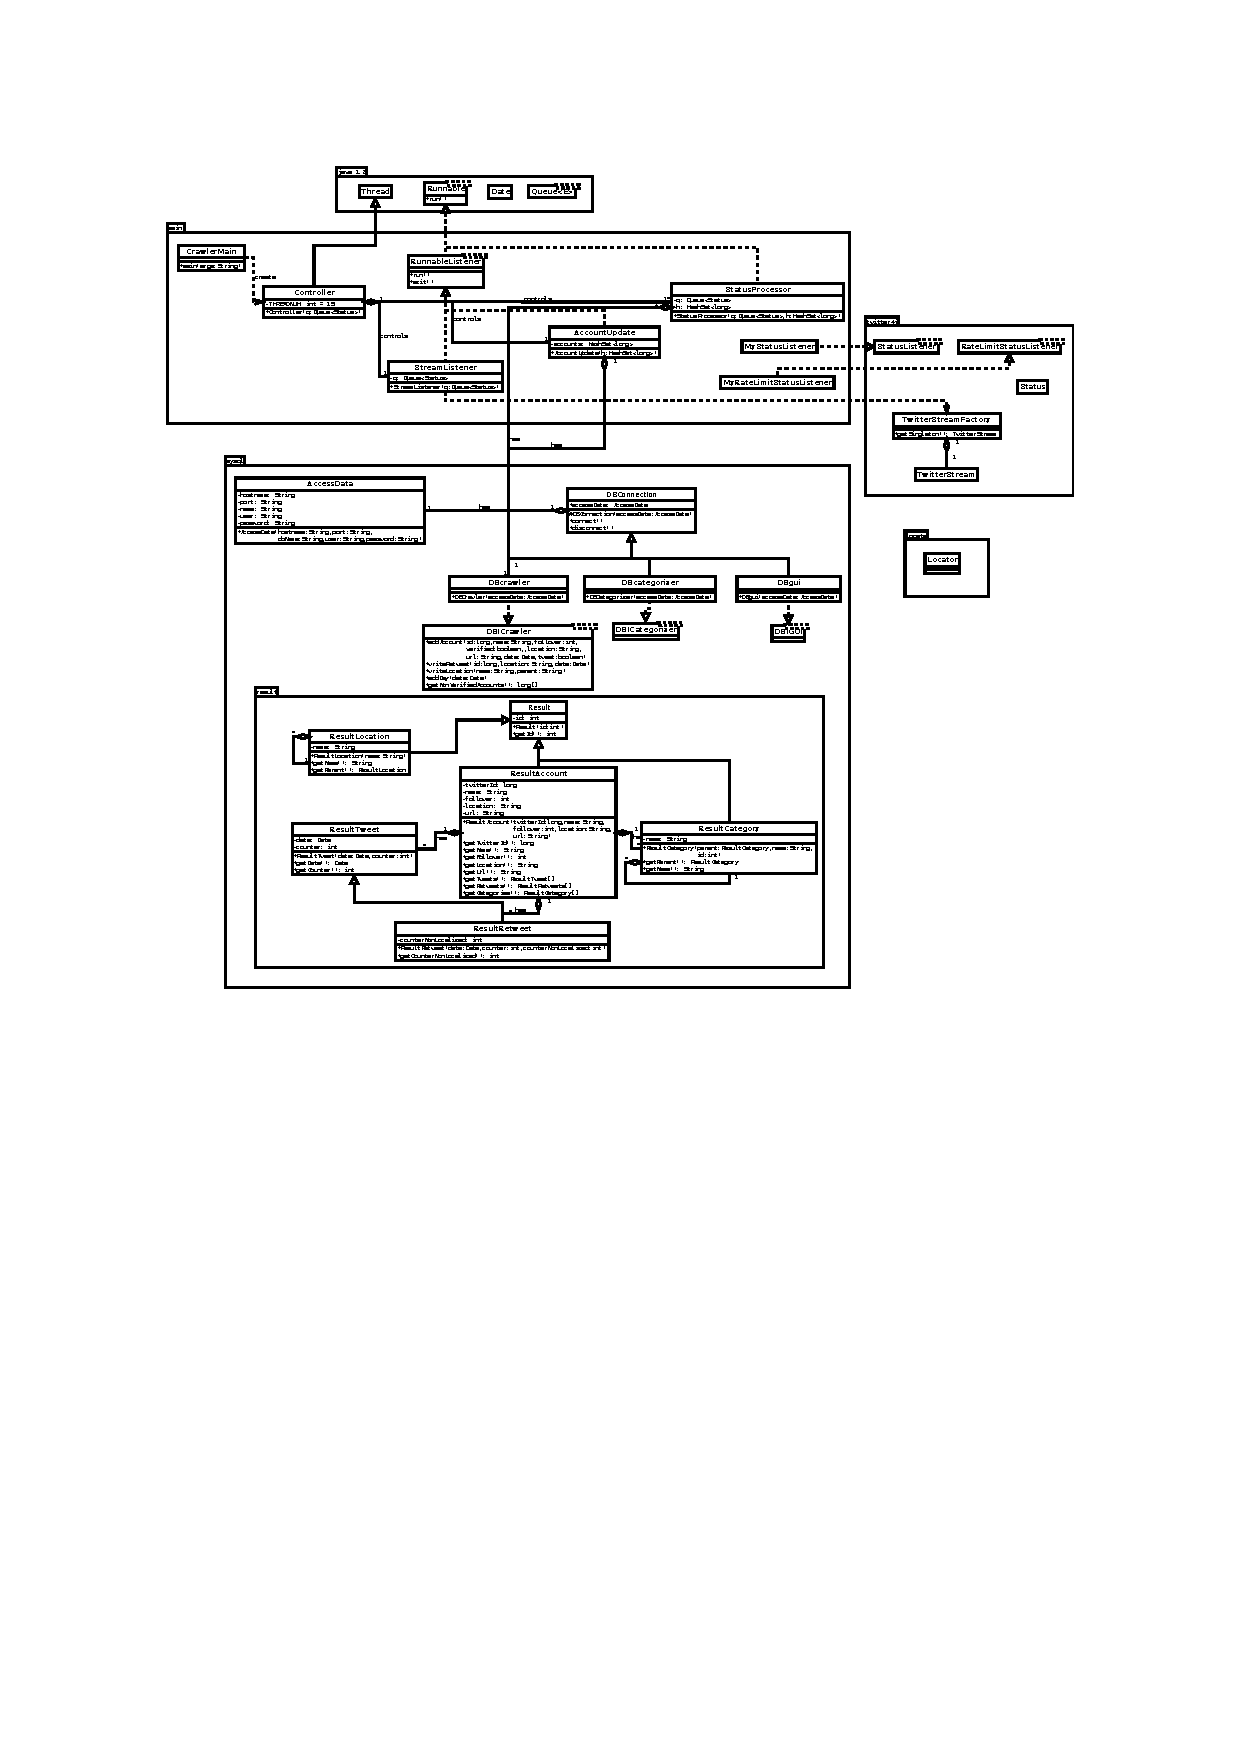
\includegraphics[height=\textwidth, width=\textheight, keepaspectratio=true, angle=90]{dia/uml_crawler}
	\caption{Größeres Klassendiagramm des Crawlers}
	\label{fig:crawler_big}
\end{figure}
\begin{figure}[h!]
	\centering
	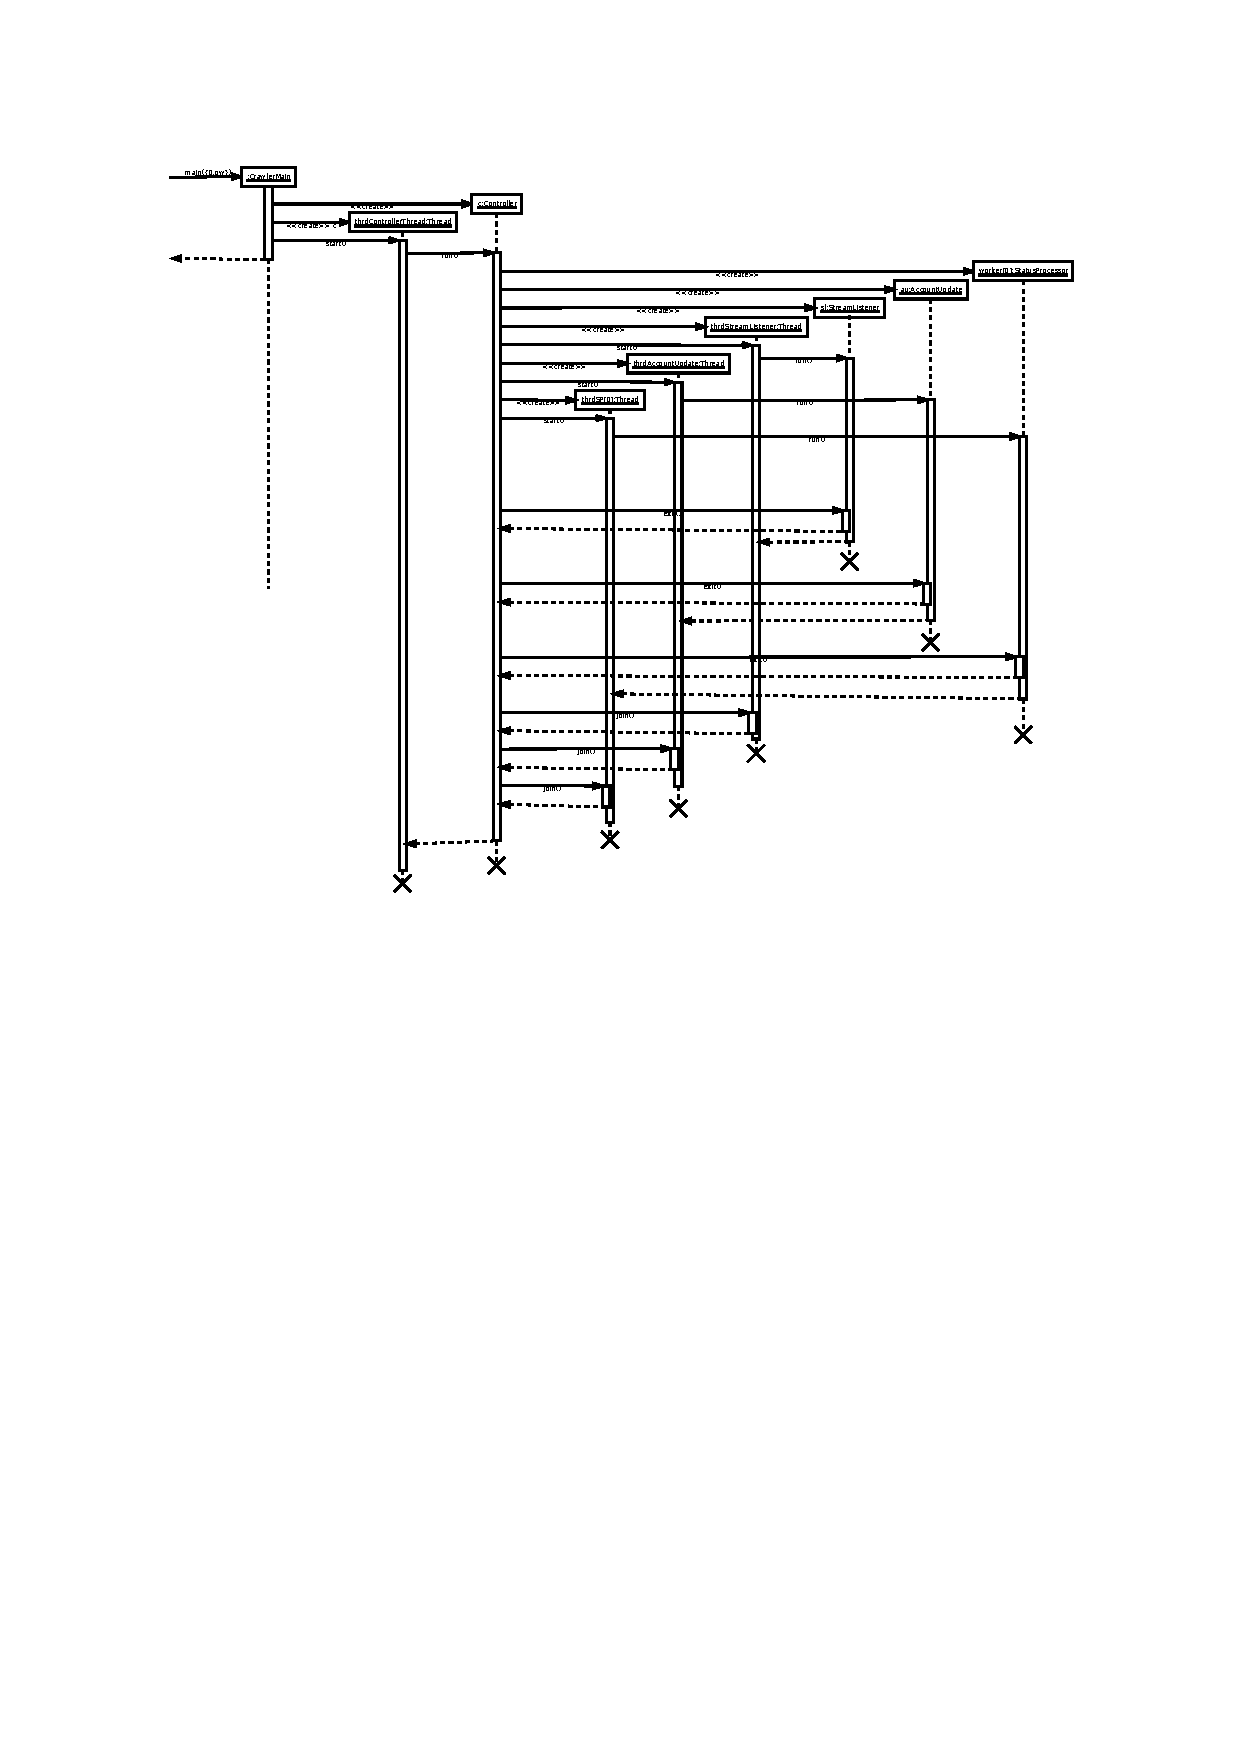
\includegraphics[height=\textwidth, width=\textheight, keepaspectratio=true, angle=90]{dia/crawler_start_sequence}
	\caption{Größeres Sequenzdiagramm des Crawler Starts}
	\label{fig:crawler_seq_big}
\end{figure}
